\begin{spacing}{1.5}
  \begin{tightcenter}
    \section{4. Implementación y pruebas}
    \mylinespacing
  \end{tightcenter}

  \subsection{4.1 Implementando tecnologías}

  \textbf{Procedimiento}

  \textbf{Anexo No.1: Instalación y configuración de los computadores de la
    sala
    de cómputo}

  En este documento se registra el proceso de instalación y configuración de
  los
  computadores de la sala de cómputo de Jürgen Tischer, Departamento de
  Matemáticas, Universidad del Valle, Cali, Colombia. Además, se detallan las
  herramientas disponibles y su utilidad.

  El documento completo de instalación y configuración se encuentra en la
  sección
  de Anexos

  \subsection{4.2 Pruebas de control}

  En el proceso de verificar el correcto funcionamiento de los computadores y
  las
  integraciones, se emplean diversas herramientas, como las presentadas a
  continuación.

  \subsubsection {4.2.1 Comprobar conectividad básica con pdsh}

  El comando \code{alias} se configuró para verificar el estado de los equipos
  en
  el clúster. Este comando permite lanzar un comando de manera más sencilla,
  por
  ejemplo, \code{pdsh xeon "hostname"}, que devuelve el nombre de
  todos los
  equipos encendidos y conectados correctamente por ssh. Además, si se utiliza
  el
  argumento \code{uptime} en vez de \code{hostname}, se puede obtener más
  información sobre el estado de cada nodo.

  \subsubsection {4.2.2 Comprobar funcionamiento en Mathematica}

  En Mathematica es fácil comprobar que la configuración paralela funciona
  correctamente. Para hacerlo, seleccione una configuración sencilla que
  incluya
  todos los nodos que desea utilizar. En nuestro caso, configuramos Lightweight
  Grid en las opciones de configuración paralela del kernel, con un kernel
  disponible para cada nodo. También es necesario desactivar
  \textit{RemoteKernel
    Objects}, que es un configurador automático que, por defecto, solo usa los
  kernels locales e ignora toda la configuración que se le coloca. Los kernels
  configurados se muestran en la Figura \ref{fig:etiqueta}.  \newline  \newline

  \begin{figure}[h]
    \centering
    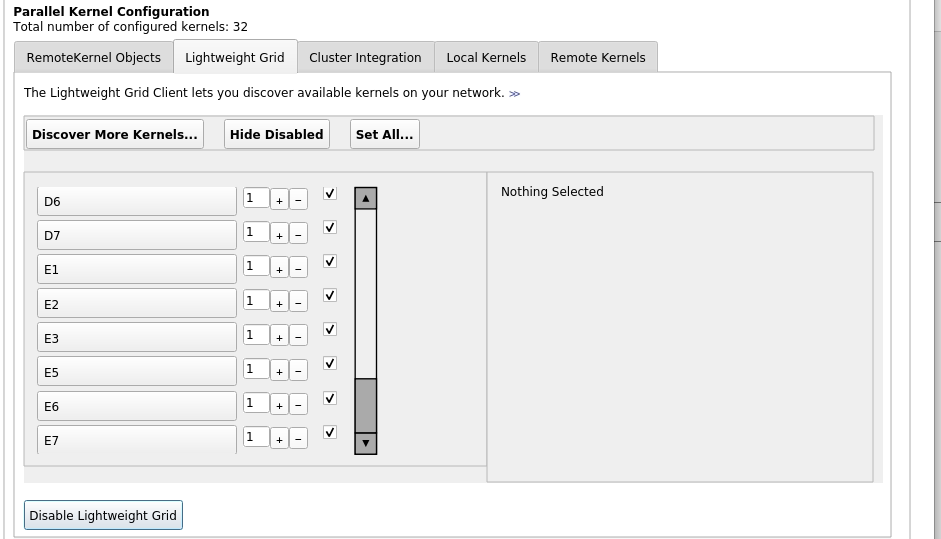
\includegraphics[width=0.9\textwidth]{mat.png}
    \caption{Configuración paralela en Mathematica}
    \label{fig:etiqueta}
  \end{figure}

  Una vez que se haya completado esta configuración, podrás abrir un nuevo
  cuaderno (notebook) y escribir la siguiente instrucción: \code{LaunchKernels[
      ]}. De esta manera, la aplicación tratará de conectarse con los kernels
  configurados en cada nodo, tal como se muestra en la Figura
  \ref{fig:etiqueta}

  \begin{figure}[h]
    \centering
    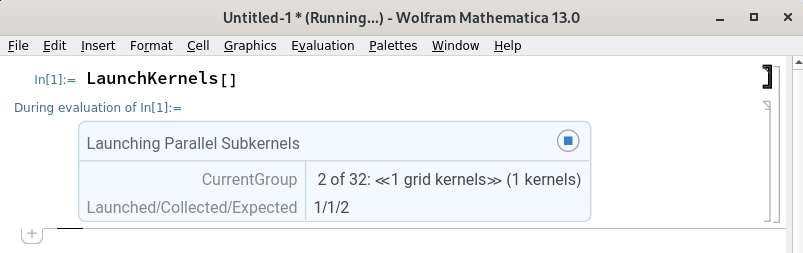
\includegraphics[width=0.9\textwidth]{mat1.png}
    \caption{Conexión de kernels y nodos}
    \label{fig:etiqueta}
  \end{figure}

  En caso de que todo salga bien, se muestra una lista con todos los kernels
  iniciados, como se indica en la Figura \ref{fig:etiqueta}

  \begin{figure}[h]
    \centering
    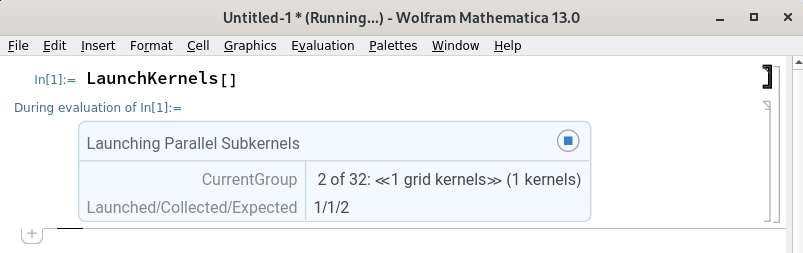
\includegraphics[width=0.9\textwidth]{mat4.png}
    \caption{Kenerls iniciados}
    \label{fig:etiqueta}
  \end{figure}

  Si hay un error, Mathematica lo señalará. Normalmente el error incluirá
  información sobre el nodo que presenta problemas, así como una breve
  descripción del problema y posibles soluciones a aplicar, en la Figura
  \ref{fig:etiqueta} se puede observa un error en Mathematica.

  \begin{figure}[h]
    \centering
    
\includegraphics[width=0.9\textwidth]{mat3.png}
    \caption{Información de error}
    \label{fig:etiqueta}
  \end{figure}

  \subsubsection {4.2.3 Comprobar funcionamiento en Slurm}

  En Slurm, hay varios comandos básicos que nos permiten ver información sobre
  el
  estado de los nodos configurados.

  \begin{itemize}
    \item \textbf{sinfo}: Muestra el estado de los nodos. Es la primera
          herramienta que se debe utilizar para visualizar si hay algún
          problema de
          comunicación con los nodos.
    \item \textbf{srun}: Agrega una tarea a la cola de manera activa.
    \item \textbf{squeue}: Muestra la lista de tareas en cola, tanto pendientes
          como en ejecución.
    \item \textbf{scancel}: Cancela una tarea que se encuentra en la cola.
    \item \textbf{scontrol}: Se utiliza principalmente para cambiar el estado
          de los nodos.
  \end{itemize}

  Es posible probar rápidamente el funcionamiento de los nodos con \code{srun},
  de manera similar a como se utilizaba \code{pdsh}. En este caso, el comando
  utilizado es \code{srun -N10 hostname}. Esto solicitará a 10 nodos
  disponibles
  que ejecuten el comando \code{hostname}, devolviendo sus nombres. Si se
  utiliza
  el número total de nodos y todos devuelven su nombre, entonces la
  comunicación
  básica funciona. Sin embargo, solo esta prueba no es suficiente para
  determinar
  un problema de sincronización, ya que puede haber un problema en la
  comunicación del número de nodos en la tarea, donde cada nodo cree que es el
  único que ejecuta la tarea y no se da cuenta de que hay otros.

  \textbf{Helloworld Paralelo con C y C++}

  Para verificar la comunicación completa, se utilizó el programa de ``hola
  mundo''
  en paralelo con MPI, escrito en C. Esto se basa en el tutorial de
  mpitutorial.com \cite{HelloC}:

  \definecolor{codebackground}{RGB}{240,240,240}
  % Color de fondo del código
  \definecolor{codecomment}{RGB}{100,100,100}
  % Color de los comentarios
  \definecolor{codekeyword}{RGB}{0,0,255}
  % Color de las palabras clave
  \definecolor{codestring}{RGB}{163,21,21}
  % Color de las cadenas de texto

  \lstset{
    backgroundcolor=\color{codebackground},
    commentstyle=\color{codecomment},
    keywordstyle=\color{codekeyword},
    stringstyle=\color{codestring},
    basicstyle=\footnotesize\ttfamily,
    breakatwhitespace=false,
    breaklines=true,
    captionpos=b,
    frame=single,
    numberstyle=\tiny\color{codecomment},
    showspaces=false,
    showstringspaces=false,
    showtabs=false,
    tabsize=2,
    rulecolor=\color{codebackground}
  }

  \begin{lstlisting}[language=C]
    #include <stdio.h>
    #include <unistd.h>
    #include <mpi.h>
    
    int main(int argc, char** argv)
    {
      // Init the MPI environment
      MPI_Init(NULL, NULL);
      // Get the number of processes
      int world_size;
      MPI_Comm_size(MPI_COMM_WORLD, &world_size);
      // Get the rank of the process
      int world_rank;
      MPI_Comm_rank(MPI_COMM_WORLD, &world_rank);
      // Get the name of the processor
      char processor_name[MPI_MAX_PROCESSOR_NAME];
      int name_len;
      MPI_Get_processor_name(processor_name, &name_len);
      // Print a hello world message
      printf("Hello, World! from node %s, rank %d out of %d processors\n",
             processor_name, world_rank + 1, world_size);
      // Finalize the MPI environment
      MPI_Finalize();
    }
    \end{lstlisting}

  Para compilar este código es necesario contar con mpicc. Para hacerlo, se
  debe utilizar el siguiente comando: \code{mpicc c-mpi-hello.c -o
    c-mpi-hello}.

  Luego, el archivo debe ser accesible desde todas las máquinas en la misma
  ubicación. Para lograr esto, se utilizó un NFS, tal como se indica en la guía
  adjunta en el apartado NFS.

  Para ejecutar el código, se debe utilizar el comando \code{srun -N10
    /nfs/c-mpi-hello}.

  \textbf{Resultados}

  \textbf{Helloworld Paralelo con Python}
  Se puede lograr lo mismo utilizando Python. Se recomienda preparar un
  entorno utilizando conda o mamba en el NFS para que esté disponible para
  todos
  los nodos involucrados. Además, el entorno debe contener el paquete
  \code{mpi4py}. En nuestro caso, utilizamos la implementación de \code{mpich}.
  El entorno fue creado con el comando \code{conda create -p /nfs/anaconda
    anaconda mpi4py mpich}.

  Para activar el entorno durante la ejecución de cada nodo, es más
  conveniente utilizar un archivo de sbatch.

  \subsection{4.3 Pruebas de eficiencia}

  \subsection{4.4 Automatización - Facilitar el uso}

  \subsubsection{4.4.1 Scripts}

  En el desarrollo de este proyecto, se llevaron a cabo diversos scripts de
  automatización que permiten realizar tareas de mantenimiento y configuración
  de
  manera más eficiente y sistemática. Estos scripts han sido diseñados para
  optimizar procesos específicos dentro del proyecto y su implementación ha
  permitido reducir el tiempo de ejecución de tareas repetitivas y mejorar la
  calidad del trabajo.

  Estas son las funciones principales de los scripts de automatización:

  \begin{itemize}
    \item Encendido y apagado de computadores.
    \item Verificación del estado de los computadores y servicios.
    \item Actualización de software.
    \item Instalación de paquetes de software.
    \item Configuración completa de un nuevo equipo recién instalado o de
          un equipo antiguo formateado.
  \end{itemize}

  Esto permitirá minimizar las tareas comunes y de mantenimiento requeridas
  con menor esfuerzo. Además, estos scripts son altamente escalables y pueden
  ser
  adaptados para su uso en proyectos futuros, lo que representa una inversión a
  largo plazo en la mejora de la eficiencia y la calidad del trabajo.

  \subsection{4.5 Problemas encontrados}
  En el desarrollo de este proyecto, se presentaron problemas tanto previstos
  como inesperados, los cuales serán mencionados a continuación.

  \subsubsection{4.5.1 Problemas esperados}

  \begin{enumerate}
    \item \textbf{Heterogeneidad de los recursos computacionales:} El clúster
          Bochica y la sala de computación Jürgen Tischer contienen una
          variedad de
          recursos computacionales, incluyendo diferentes tipos de
          computadoras, sistemas
          operativos y versiones de software. Esto puede dificultar la
          optimización del
          sistema distribuido diseñado y requerir una mayor planificación y
          flexibilidad
          en el diseño y la implementación.
    \item \textbf{Antigüedad de los computadores:} Algunos de los computadores
          en el clúster Bochica y la sala de computación Jürgen Tischer son
          antiguos y
          pueden tener un impacto en la eficiencia y la capacidad de ejecutar
          tareas de
          investigación de manera óptima.
    \item \textbf{Dificultades en la adaptación a las nuevas herramientas:} La
          implementación de nuevas herramientas y tecnologías puede requerir un
          período
          de adaptación y aprendizaje para los usuarios, lo que puede retrasar
          los
          procesos de investigación y enseñanza. Además, pueden surgir
          problemas técnicos
          durante la instalación y configuración de las herramientas, lo que
          puede
          interferir en la eficiencia y productividad.
  \end{enumerate}

  \subsubsection{4.5.2 Problemas no esperados}

  \textbf{Problemas con el software}

  \begin{itemize}
    \item Problemas de licencias: Parte del software utilizado era
          propietario y resultó problematico el correcto uso de estas
          licencias,
          especialmente el software de Wolfram Mathematica.
  \end{itemize}

  \textbf{Problemas con el hardward}

  \begin{itemize}
    \item Cables mal acomodados: Los cables del clúster estaban mal
          acomodados, lo que generaba una dificultad para conocer las
          diferentes
          interconexiones entre los recursos.
    \item Cables faltantes: Se encontró que se requería un cable serial
          para la adecuada configuración de un switch que permite la
          interconexión entre
          los equipos del clúster.
    \item Permisos olvidados: Varios equipos del clúster debido a su
          desuso, se habían perdido las credenciales para utilizarlos de la
          manera
          adecuada
    \item Partes que requerían mantenimiento: Algunas partes del hardware
          requerían mantenimiento para su óptimo funcionamiento, pero esto no
          se había
          realizado.
    \item Desconocimiento de las limitaciones del hardware: Al principio no
          se conocían las limitaciones del hardware, lo que dificultaba su
          correcto uso y
          aprovechamiento.
    \item Hardware mal acomodado: El hardware estaba mal acomodado, lo que
          generaba problemas en la conexión y en el acceso a los recursos
          computacionales.
  \end{itemize}

  \textbf{Problemas con la Implementación del Sistema Distribuido}

  \begin{itemize}
    \item Falta de documentación clara para la implementación: La
          documentación para la implementación del sistema distribuido no era
          clara, lo
          que dificultaba su correcta implementación.
    \item Dificultades en la integración de los diferentes componentes del
          sistema: Se encontraron dificultades en la integración de los
          diferentes
          componentes del sistema distribuido, lo que limitaba su correcto
          funcionamiento.
    \item Limitaciones en la capacidad de paralelización: Se encontraron
          limitaciones en la capacidad de paralelización del sistema
          distribuido, lo que
          disminuía su eficiencia y efectividad.
  \end{itemize}

  \textbf{Problemas con las Herramientas Instaladas}

  \begin{itemize}
    \item Falta de compatibilidad con otras aplicaciones: Las herramientas
          instaladas no eran compatibles con otras aplicaciones, lo que
          limitaba su uso y
          efectividad.
    \item Dificultades en la configuración y uso: Se encontraron
          dificultades en la configuración y uso de las herramientas
          instaladas, lo que
          disminuía su efectividad.
    \item Falta de documentación y apoyo técnico: La falta de documentación
          y apoyo técnico para las herramientas instaladas limitaba su uso y
          efectividad.
  \end{itemize}

  \textbf{Problemas con las Pruebas de Rendimiento}

  \begin{itemize}
    \item Falta de recursos y tiempo para realizar las pruebas: No se
          contaba con los recursos y tiempo necesario para realizar las pruebas
          de
          rendimiento, lo que limitaba la evaluación de la infraestructura y
          las
          aplicaciones implementadas.
    \item Falta de una metodología clara para la realización de las
          pruebas: No había una metodología clara para la realización de las
          pruebas de
          rendimiento, lo que generaba incertidumbre en los resultados y
          dificultades en
          la interpretación de los mismos.
    \item Dificultades en la comparación de resultados con otras
          infraestructuras: Se encontraron dificultades en la comparación de
          los
          resultados obtenidos con otras infraestructuras similares, lo que
          disminuía la
          validez de los resultados.
    \item Falta de un sistema de seguimiento y monitoreo de las pruebas: No
          había un sistema de seguimiento y monitoreo de las pruebas, lo que
          dificultaba
          la identificación y solución de posibles problemas y limitaba la
          mejora
          continua de la infraestructura.
  \end{itemize}

  \mylinespacing
  \mylinespacing
  \begin{tightcenter}
  \end{tightcenter}
\end{spacing}